

\chapter{Se repérer dans l'espace}


\section{Le système de coordonnées}


\subsection{Le repère ''main droite''}

Le repère est orthogonal et orthonormé (les axes/les vecteurs directeurs de ces axes sont perpendiculaires les uns aux autres et de longueur 1)



\subsection{Pourquoi main droite ?}

Regardez votre main droite.
\begin{itemize} 
\item Votre pouce représente l'axe X, 
\item votre index représente l'axe Y,
\item votre majeur représente l'axe Z. 
\end{itemize}

La direction dans laquelle pointe chacun de vos doigts définit le sens de chaque axe.

Image utilisateur cf(\url{fr.openclassrooms.com/informatique/cours/decouvrez-ogre-3d/le-systeme-de-coordonnees-1})





\subsection{Repère local, repère absolu}

Pour l'instant, nous n'avons toujours pas défini comment le repère était placé dans la scène. C'est une question de convention adoptée pour les applications 3D	pour le repère de la scène:
\begin{itemize}
\item l'axe Y dirigé vers le haut 
\item les axes X et Z dans un plan horizontal.
\end{itemize}

Seulement\footnote{comment faire pour sauter une ligne avant le ''Seulement''?}, la scène n'est pas la seule à avoir son repère. En effet, chaque objet possède son propre repère appelé repère local. Lorsque l'objet se déplace ou tourne sur lui-même, le repère local fait de même. L'orientation du repère local est la suivante: 
\begin{itemize}
\item l'axe Y est dirigé vers le haut de l'objet, pour la scène, 
\item l'axe X est dirigé vers sa droite
\item l'axe Z vers l'arrière de l'objet.
\end{itemize}
	


Ci-dessous\footnote{comment faire pour sauter une ligne avant le ''Ci-dessous''?}, j'ai représenté en noir le repère de la scène, et en bleu le repère local de la voiture, en respectant la convention que j'ai donnée.
Image utilisateur cf(\url{fr.openclassrooms.com/informatique/cours/decouvrez-ogre-3d/le-systeme-de-coordonnees-1})

Nous verrons à quoi servent ces différents repères lorsque l'on commencera à déplacer nos objets.








\subsection{Yaw, pitch, roll}

yaw pitch roll sont les désignations anglaises pour les rotations autour des axes Y, X et Z respectivement. On peut traduire ces termes par lacet (yaw), tangage (pitch) et roulis (roll), qui sont utilisés par exemple en aéronautique ou en navigation.

Ces trois termes se retrouveront dans les noms qu'Ogre donne aux méthodes permettant d'effectuer des rotations. 

Voici tout de suite un schéma illustrant les rotations qui s'appliquent à chaque axe:

Image utilisateur cf(\url{fr.openclassrooms.com/informatique/cours/decouvrez-ogre-3d/le-systeme-de-coordonnees-1})


Tout comme l'orientation des axes de notre repère, il y a un sens direct et un sens indirect pour les rotations! Vous tournerez dans le sens direct lors  d'une rotation contraire\footnote{''rotation contraire'' <-> ''sens direct'', est ce correct?} au sens des aiguilles d'une montre.

Pour effectuer une rotation, on appelle la méthode correspondante pour le noeud:
\begin{lstlisting}
	node->yaw(Radian(Math::PI));
\end{lstlisting}

Ceci fera faire un demi-tour au noeud par rapport à son axe vertical tandis que les méthodes pitch() et roll() s'utilisent de fa\c{c}on analogue pour les autres axes.

La rotation se fait par défaut par rapport au repère local. Il faut renseigner le second paramètre si vous voulez qu'il en soit autrement (voir la section suivante).

Les angles doivent être entrés en radians. Pour utiliser tout de même des degrés dans Ogre, vous devrez utiliser la classe Degree. La ligne de code précédente est équivalente à ceci:
\begin{lstlisting}
	node->yaw(Degree(180));
\end{lstlisting}









\section{Déplacer des objets}




\subsection{Bouger un noeud de scène}

Nous allons maintenant déplacer notre tête d'ogre pour vérifier la théorie et enfin sortir notre tête de terre!

Pour cela, nous allons donc passer par le noeud auquel est rattaché notre mesh. Celui-ci possède deux méthodes qui peuvent nous servir.




\subsection{setPosition()}

La méthode setPosition() prend en paramètres les trois coordonnées X, Y et Z du point auquel on désire placer le noeud. On peut aussi lui passer un Vector3, qui contiendra lui-même ces coordonnées.

Les deux codes suivants sont donc équivalents.
\begin{lstlisting}
	Vector3 position = Vector3(30.0, 50.0, 0.0);
	node->setPosition(position);
\end{lstlisting}

ou
\begin{lstlisting}
	node->setPosition(30.0, 50.0, 0.0);
\end{lstlisting}

La tête s'est maintenant déplacée vers la droite de 30 unités et de 50 unités vers le haut.




\subsection{translate()}

La méthode translate() déplace le noeud par rapport à sa position actuelle plutôt que par rapport à l'origine de la scène.

Elle prend les mêmes paramètres que la méthode setPosition(), mais avec un paramètre supplémentaire, défini par défaut, indiquant le noeud par rapport auquel on va se déplacer.
\begin{lstlisting}
	node->translate(-30.0, 50.0, 0.0);
\end{lstlisting}

En ajoutant cette ligne après la précédente, notre objet se retrouve donc maintenant à la position (0, 100, 0) dans la scène, ce qui est suffisant pour qu'il surplombe son petit jardin.

Image utilisateur

Le paramètre supplémentaire (par rapport à setPosition) permet de définir par rapport à quel repère on va déplacer le noeud.

Les trois valeurs possibles sont:
\begin{lstlisting}
    Node::TS_LOCAL //va deplacer le noeud par rapport au repere local
    Node::TS_PARENT //va deplacer le noeud au repere du noeud parent
    Node::TS_WORLD //va deplacer le noeud au repere de la scene, qui est le repere absolu.
\end{lstlisting}\footnote{Pour présenter les 3 valeurs possibles ne devrais je pas faire une liste itemize plutôt que d'utiliser un bloc de code?}



\subsection{Concrètement, \c{c}a veut dire quoi ?}

Tout à l'heure, lorsque l'on a effectué une translation, on l'a fait par défaut par rapport au repère TS\_WORLD, c'est-à-dire avec les axes tels que je vous les ai présentés précédemment. Maintenant, nous pouvons déplacer notre noeud par rapport au repère local de son noeud père par exemple, ou bien même par rapport à son propre repère local.

Mais à quoi \c{c}a sert de s'embêter avec ces paramètres ? On risque de faire des erreurs si l'on se place par rapport à un repère différent de la scène!

Prenons un exemple. Vous avez un vaisseau spatial qui peut se trouver dans n'importe quelles position et orientation de l'espace. Comment savoir facilement dans quelle direction je dois faire ma translation pour qu'on le voit aller en avant ?

Réponse: je n'ai pas à m'en occuper! En effet, l'axe qui va de l'avant vers l'arrière du vaisseau est l'axe Z, dans son repère local. Par conséquent, je n'ai qu'à dire à mon vaisseau d'avancer le long de l'axe Z (dans le sens négatif pour aller à l'avant) par rapport à son repère local. Et Ogre s'occupera gentiment de faire les calculs pour placer mon vaisseau correctement dans la scène.

Image utilisateur \url{http://fr.openclassrooms.com/informatique/cours/decouvrez-ogre-3d/deplacer-des-objets}

Si vous avez compris cela, le paramètre TS\_PARENT devrait suivre tout seul. Reprenons notre engin spatial.
Sur ce vaisseau, on trouve R2D2 en train de se déplacer vers la droite, correspondant donc à l'axe X local du noeud du vaisseau. Pour effectuer cette translation, je n'ai qu'à demander à Ogre de déplacer mon robot le long de l'axe des abscisses par rapport au noeud du vaisseau (qui serait logiquement le noeud parent).

Vous commencez à comprendre l'intérêt des relations de parenté entre les noeuds ?









\section{La caméra}


La caméra, c'est l'élément qui définit la position de notre point de vue dans la scène, dans quelle direction on regarde, mais aussi jusqu'à quelle distance il est possible de voir s'afficher les objets éloignés.

Comme tous les éléments de base, un attribut caméra est présent dans la classe ExampleApplication. Sans elle nous n'aurions pas encore pu voir notre scène, vu que nous n'avons rien fait pour la créer!



\subsection{Création}

La caméra est créée par la méthode  createCamera() de la classe ExampleApplication, nous allons tout de suite redéfinir cette méthode pour partir sur des bases connues. L'attribut correspondant à la caméra est appelé mCamera, nous pouvons donc l'utiliser pour créer notre caméra.

Comme c'est un objet qui se trouve dans la scène, nous allons passer par le sceneManager. Comme pour les noeuds ou les entités, vous pourrez donner un nom à votre caméra sous forme d'une cha\^ine de caractères.

Ajoutez la méthode createCamera() à votre classe PremiereApplication et ajoutez-y la ligne suivante.

\begin{lstlisting}
	mCamera = msceneMgr->createCamera(''Ma Camera'');
\end{lstlisting}





\subsection{Placement}

Maintenant, il va nous falloir placer la caméra et l'orienter. Le placement se fait avec la méthode setPosition(). 

La seconde méthode utilisée s'appelle lookAt() et, comme son nom l'indique, elle permet de déterminer le point de la scène que regarde notre caméra. On lui fournit un Vector3 ou bien trois réels correspondant aux coordonnées désirées.

\begin{lstlisting}
	//placement de la camera
	mCamera->setPosition(Vector3(-100.0, 150.0, 200.0));
	//point de la scene que regarde notre camera
	mCamera->lookAt(Vector3(0.0, 100.0, 0.0));
\end{lstlisting}


Enfin, on peut aussi indiquer les distances near clip et far clip, qui sont les distances minimale et maximale\footnote{''les distances minimale et maximale'' il faut pas de ''s'' à ''max/minimale""} auxquelles doit se trouver un objet pour être affiché à l'écran.
\begin{lstlisting}
	mCamera->setNearClipDistance(1);
	mCamera->setFarClipDistance(1000);
\end{lstlisting}




\subsection{Code}

\subsubsection{PremiereApplication.cpp}
\begin{lstlisting}[caption={PremiereApplication.cpp: Création de la caméra}]

#include "PremiereApplication.h"

void PremiereApplication::createScene()
{
    //creation d une entite
    Entity *head= mSceneMgr->createEntity("Tete", "ogrehead.mesh" );
    
    //creation d un noeud
    SceneNode *node= mSceneMgr->getRootSceneNode( )->createChildSceneNode( "nodeTete " , Vector3::ZERO, Quaternion::IDENTITY);
    
    node->yaw(Radian(Math::PI));
    node->yaw(Radian(Math::PI));

    //setPosition place le noeud aux coord passees en parametres
    Vector3 position = Vector3(30.0, 50.0, 0.0);
    node->setPosition(position);

    node->setPosition(30.0, 50.0, 0.0); 
    /*equivalent a
    Vector3 position = Vector3(30.0, 50.0, 0.0);
    node->setPosition(position);
    */

    //deplace le noeud par rapport a sa position actuelle
    node->translate(-30.0, 50.0, 0.0); //par defaut la trnslt se fait par rap a TS_WORLD
   
    //attachement de l entite au noeud
    node->attachObject ( head );

    //creation d un plan
    Plane plan(Vector3::UNIT_Y, 0);

    //creation d un mesh cad l objet 3d visible ds la scene
    MeshManager::getSingleton().createPlane("sol",
                ResourceGroupManager::DEFAULT_RESOURCE_GROUP_NAME,
                plan, 500, 500, 1, 1, true, 1, 1, 1, Vector3::UNIT_Z); 

    //entite qui representera le plan
    Entity *ent= mSceneMgr->createEntity("EntiteSol", "sol");

    //ajout du materiau a l entite
    ent->setMaterialName("Examples/GrassFloor");//texture de pelouse
    /*les differents materiaux sont sous /media/materials/scritps, par ex:
    ent->setMaterialName("Examples/WaterStream");//texture d eau animee*/

    //creation d un noeud
    node = mSceneMgr->getRootSceneNode()->createChildSceneNode();
    node->attachObject(ent);
}

/*definit la position de notre point de vue*/
void PremiereApplication::createCamera()
{
    //creation de la camera
    mCamera = mSceneMgr->createCamera("Ma Camera");

    //position de la camera
    mCamera->setPosition(Vector3(-100.0, 150.0, 200.0));

    //permet de determiner le point de la scene que regarde notre camera
    mCamera->lookAt(Vector3(0.0, 100.0, 0.0));

    //definition des distances de near clip et de far clip, qui
    //sont les distances minimale et maximale auxquelles doit se
    //trouver un objet pour etre afficher a l'ecran.
    mCamera->setNearClipDistance(1);
    mCamera->setFarClipDistance(1000);
}

\end{lstlisting}



\subsubsection{PremiereApplication.h}
\begin{lstlisting}[caption={PremiereApplication.h: Création de la caméra}]
using namespace std;

#include <ExampleApplication.h>

class PremiereApplication : public ExampleApplication
{
public:
    void createScene();
    void createCamera();
};

\end{lstlisting}


\subsubsection{main.cpp}
\begin{lstlisting}[caption={main.cpp: Création de la caméra}]
#include <Ogre.h>

#include "PremiereApplication.h"

#if OGRE_PLATFORM == PLATFORM_WIN32 || OGRE_PLATFORM == OGRE_PLATFORM_WIN32
#define WIN32_LEAN_AND_MEAN
#include "windows.h"

INT WINAPI WinMain(HINSTANCE hInst, HINSTANCE, LPSTR strCmdLine, INT)
#else
int main(int argc, char **argv)
#endif
{

    PremiereApplication app;
    
    try {
      app.go();
    } catch(Ogre::Exception& e) {
#if OGRE_PLATFORM == OGRE_PLATFORM_WIN32
        MessageBoxA(NULL, e.getFullDescription().c_str(), "An exception has occurred!", MB_OK | MB_ICONERROR | MB_TASKMODAL);
#else
        fprintf(stderr, "An exception has occurred: %s\n",
            e.getFullDescription().c_str());
#endif
    }

    return 0;
}
\end{lstlisting}




































\section{Le viewport}

Une zone de rendu est une portion de l'écran sur laquelle est affichée ce que voit la caméra. La gestion de l'affichage dans une zone de rendu est à la charge de la classe Viewport.

Cette gestion de la zone de rendu a cela d'important que:
\begin{itemize}
\item la fa\c{c}on dont la caméra rend à l'écran ce qu'elle voit ne dépend pas que d'elle. En effet, la taille de votre zone de rendu et son format seront répercutés sur la portion de scène qu'il vous sera donné de voir. Si l'on ne tenait pas compte de ces paramètres, on pourrait obtenir une image aplatie si l'on élargissait la zone de rendu, ou bien au contraire compressée si l'on diminuait la largeur en laissant la hauteur constante.
\item sur une même écran, vous pouvez afficher le rendu de plusieurs caméras dans la scène, voire des caméras de différents sceneManager.
\end{itemize}


Nous allons redéfinir la méthode createViewports() qui s'occupait jusqu'alors de ce travail pour nous. On commence par ajouter une vue:

\begin{lstlisting}
	Viewport *vue = mWindow->addViewport(mCamera);
\end{lstlisting}

Ici, mWindow est la fenêtre de notre application Ogre, c'est une instance de la classe RenderWindow dont nous verrons les détails dans un prochain chapitre. La méthode addViewport permet donc d'ajouter une vue, seul son premier argument est obligatoire. Ce premier argument est la caméra à partir de laquelle est rendu la scène affichée dans la vue.

Nous allons faire co\"incider le rapport largeur/hauteur de notre caméra avec celui du Viewport, pour avoir une image non déformée:
\begin{lstlisting}
mCamera->setAspectRatio(Real(vue->getActualWidth()) / Real(vue->getActualHeight()));
\end{lstlisting}

On applique un cast vers le format Ogre::Real pour obtenir un ratio décimal. Dans le cas contraire, le ratio serait tronqué pour être entier et la tête de notre ogre favori serait déformée.

Sachez aussi que c'est le Viewport qui définit la couleur de fond de la scène que vous voyez. 
\begin{lstlisting}
vue->setBackgroundColour(ColourValue(0.0, 0.0, 1.0));
\end{lstlisting}

Voici donc ma méthode createViewports() au complet:
\begin{lstlisting}[caption={Création d'un viewport}]
void PremiereApplication::createViewports()
{
    Viewport *vue = mWindow->addViewport(mCamera);
    
    
    //nous faisons coincider le rapport largeur / hauteur de 
    //notre camera avec celui du Viewport, pour avoir 
    //une image non deformee
    mCamera->setAspectRatio(Real(vue->getActualWidth()) / Real(vue->getActualHeight()));
    
    //couleur de fond de la vue
    vue->setBackgroundColour(ColourValue(0.0, 0.0, 1.0));
}
\end{lstlisting}


Maintenant, notre scène possède un magnifique ciel fond bleu.









\subsection{Plusieurs viewports}
La méthode addViewport permet d'ajouter des vues à notre scène, on peut donc avoir plusieurs vues à l'écran. Pour cela il faut renseigner les autres paramètres de la méthode addViewport.\newline
Voici le \href{http://www.ogre3d.org/docs/api/1.9/classOgre_1_1RenderTarget.html#a1a558e64db9dfd7cc4cec4547fca0e39}{prototype} de la méthode addViewport.


\begin{lstlisting}[caption={Prototype de addViewport}]
virtual Viewport* Ogre::RenderTarget::addViewport(
	 	Camera *  	cam,
		int  	ZOrder = 0,
		float  	left = 0.0f,
		float  	top = 0.0f,
		float  	width = 1.0f,
		float  	height = 1.0f 
		) 
\end{lstlisting}

Les paramètres sont les suivants\footnote{d'autres essais et recherches seraient nécessaires pour la pleine compréhension de ces paramètres}:
\begin{itemize}
\item ZOrder: ordre relatif des vues les unes par rapport aux autres, les Z-orders les plus élevés sont au-dessus des autres. Le nombre donnée est pas important en lui-même car il s'agit d'une relation avec les autres Z-order, ainsi peut-on utiliser des nombres qui ne suivent pas.
\item left: la position relative de la gauche du viewport sur la cible\footnote{''cible'' est visiblement le viewport principal} (entre 0 et 1).
\item top: la position relative du haut du viewport sur la cible (entre 0 et 1).
\item width: la largeur relative du viewport sur la cible (entre 0 et 1).
\item height: la hauteur relative du viewport sur la cible (entre 0 et 1).
\end{itemize}


	
\subsubsection{Code: 2 vues}
Le code suivant permet la création de deux viewports:


\begin{lstlisting}[caption={createViewports: création de plusieurs vues}]
void PremiereApplication::createViewports()
{
    //la creation du Viewport "principal"
    Viewport *vue = mWindow->addViewport(mCamera, 0, 0, 0, 0.8, 0.8);
    mCamera->setAspectRatio(Real(vue->getActualWidth()) /  Real(vue->getActualHeight()));
    vue->setBackgroundColour(ColourValue(0.980, 0.502, 0.447)); //saumon

   // creation d'un second viewport
   Viewport* vue2 = mWindow->addViewport(mCamera, 1, 0.5, 0, 0.2, 0.2);
   vue2->setBackgroundColour(ColourValue(0.561, 0.737, 0.561 ));  //darkseagreen
}
\end{lstlisting}

Et j'obtiens:
	\begin{center}
	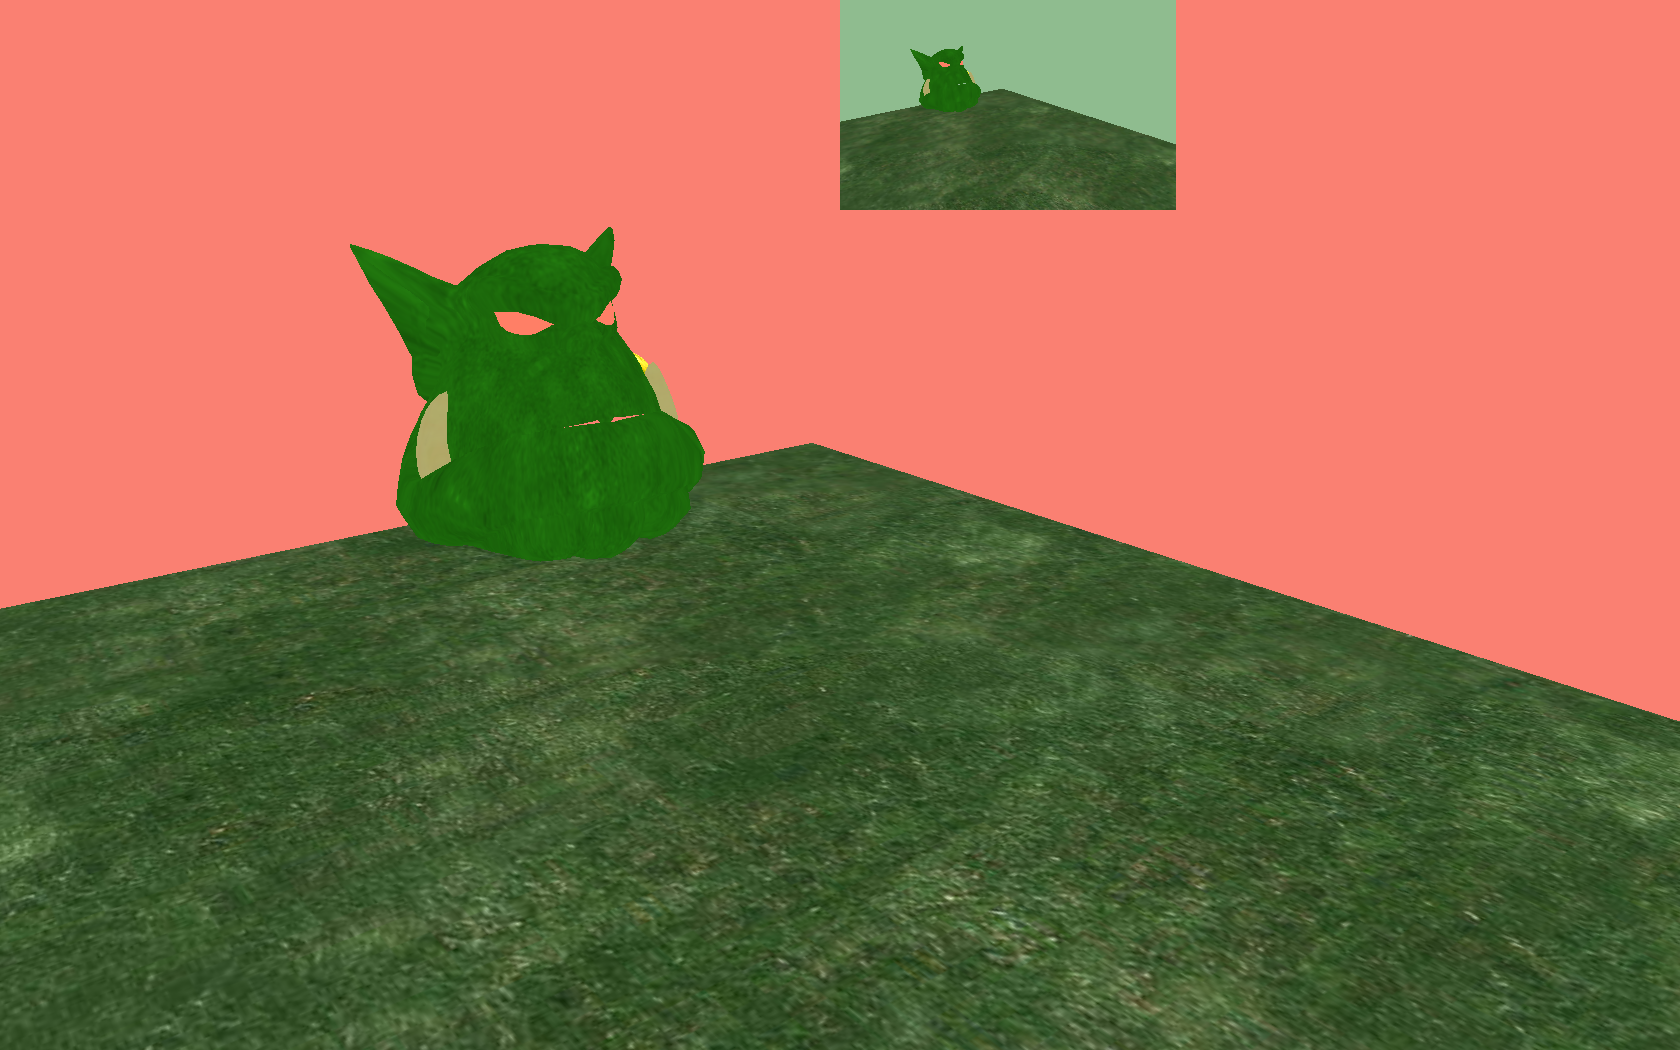
\includegraphics[scale=0.25]{Ogre/1_Base_de_Ogre/2_Se_reperer_ds_l_espace/Images/plusieursViewport.png} 
	\end{center}






\subsubsection{Code: 3 vues}
Le code suivant permet la création de deux viewports:


\begin{lstlisting}[caption={createViewports: création de plusieurs vues}]

void PremiereApplication::createViewports()
{
    //Viewport "principal"
    Viewport *vue = mWindow->addViewport(mCamera);
    mCamera->setAspectRatio(Real(vue->getActualWidth()) /  Real(vue->getActualHeight()));
    vue->setBackgroundColour(ColourValue(0.980, 0.502, 0.447)); //saumon

	//seconde vue
    Viewport* vue2 = mWindow->addViewport(mCamera, 1, 0.5, 0, 0.8, 0.8);
    vue2->setBackgroundColour(ColourValue(0.561, 0.737, 0.561 ));  //darkseagreen

	//troisieme vue
	Viewport* vue3 = mWindow->addViewport(mCamera, 4, 0, 0.4, 0.2, 0.2);
    vue3->setBackgroundColour(ColourValue(0.878, 1.000, 1.000));  //
}
\end{lstlisting}

Et j'obtiens:
	\begin{center}
	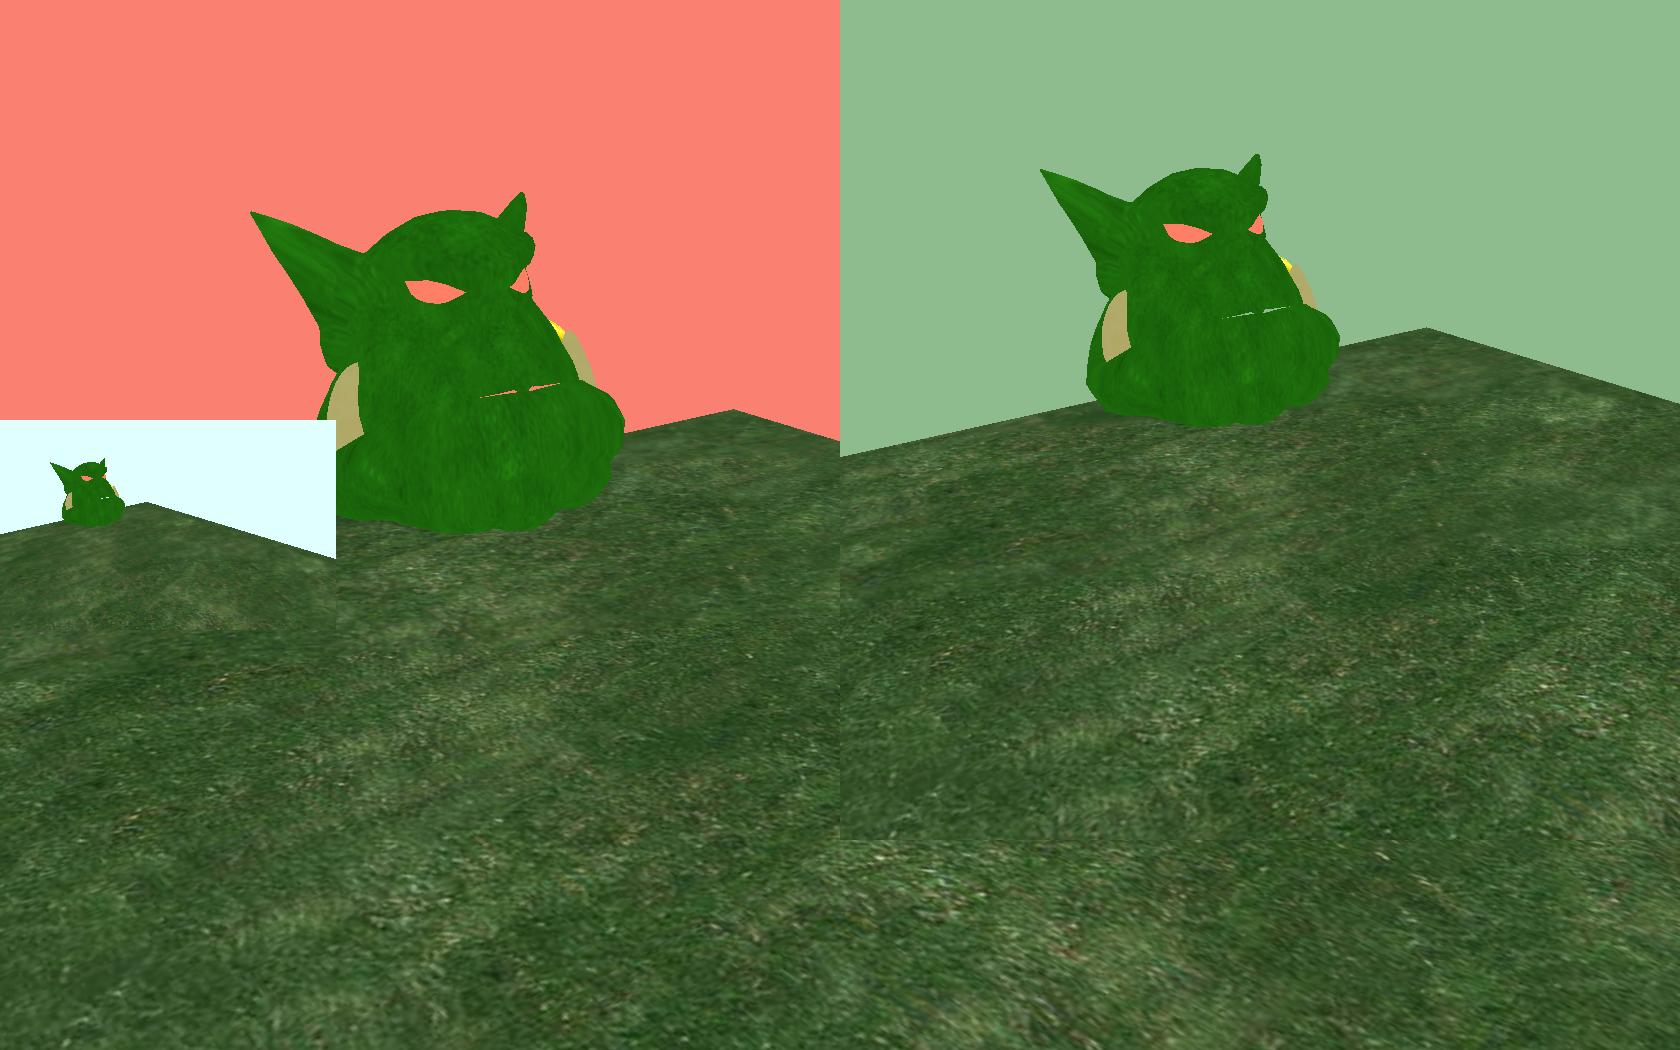
\includegraphics[scale=0.25]{Ogre/1_Base_de_Ogre/2_Se_reperer_ds_l_espace/Images/plusieursViewport2.png} 
	\end{center}
